\subsection{支持向量机对脑电信号的模式识别}
上述分析的结果主要将关注点集中在了单个通道或者单个脑区上。
而计时的理论之一就提到了群体放电的模式可能参与了时间的编码\cite{remington2018dynamical}。
相比与单个通道或者单个脑区对时间的编码,群体的放电模式有着更多的可能性,
容错的能力也更强。
虽然过去群体放电的理论模型通常采用更精细化的电生理数据,即单细胞层面的放电频率,
但由于本课题中技术手段的限制,我们无法对人进行单细胞层面的记录,因而对不同通道
的局部场电位的放电模式进行分析。

我们首先将能量曲线的数据(图\ref{fig:ephys_example}~d)做进一步的分割,
以光栅刺激开始的时刻作为零点,将时间分为20~份,每份250~毫秒;
对每份时间求其平均的能量强度(图\ref{fig:svm}~a)。
接着,我们采用留一验证(leave-one-out cross validation)的方式对数据集进行
支持向量机的学习分类。每个时间点支持向量机都会给出其对应20份时间点的概率;
我们选择其中概率最高的时间点作为其支持向量机的输出(图\ref{fig:svm}~a)。
我们再将7天实验不同次刺激的结果汇总,统计各个时刻点得到的支持向量机输出,
得到支持向量机对应结果的热力图(图\ref{fig:svm}~b)。
可以看到,在光栅刺激结束之后,仍有数个时间节点保持了放电模式的一致性。
但在一定时长后,这种特定的放电模式就区域混乱而无法被支持向量机很好的分类。
% 随机对照说明
为了避免结果存在过拟合的情况,我们增加了两组随机对照:
测试随机(图\ref{fig:svm}~c)和时间随机(图\ref{fig:svm}~d)。
可见时间随机的结果为完全随机,提示支持向量机不存在过拟合现象。
而测试随机的结果比没随机前线性相关系数有所提升,
提示在记录过程中存在我们未能控制的“噪音”信息。

\begin{figure}[h]
    \centering
    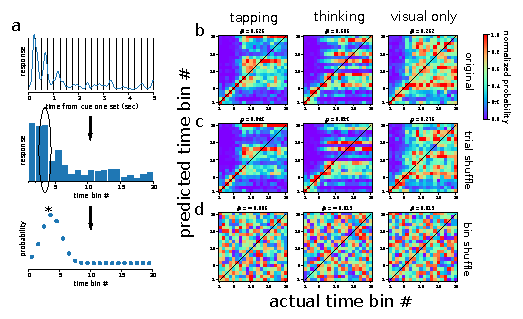
\includegraphics[width=\textwidth]{src/figures/svm.pdf}
    \caption{\textbf{支持向量机对脑电信号的模式识别}\\
    (\textbf{a})~分析流程。将单个通道一次刺激的能量曲线分为20份,
    计算每份的平均能量。将多个通道的所有数据进行支持向量机分析,
    得到某一份时间对应的概率分布,选取其中最大概率的点作为输出。
    例如图中的黑圈实际为第3份时刻,而支持向量机的输出为第4份时刻。
    (\textbf{b})~对三种范式的视觉皮层通道进行支持向量机分析。
    \(\rho\)为线性相关系数。(\textbf{c})~将数据集进行测试随机后
    的输出结果。(\textbf{d})~将数据集进行时间随机后的输出结果。
    热图的概率分布经过了对列的归一化处理。}
    \label{fig:svm}
\end{figure}

